\newcommand{\meanPerSampleScores}{
    \begin{table}[H]
        \centering
        \begin{tabular}{|P{3,2cm}||P{1,8cm} P{1,8cm} P{1,8cm} P{1,8cm} P{1,8cm}|}
            \hline
            Mean per-sample & \multicolumn{5}{c|}{\textbf{FPR}} \\
            tagging scores & $10^{-5}$ & $10^{-4}$ & $10^{-3}$ & $10^{-2}$ & $10^{-1}$ \\
            \hline
            \multicolumn{6}{|c|}{\textbf{Jaccard Similarity}} \\
            \hline
            ALOHA & 0.718$\pm$0.000 & 0.718$\pm$0.000 & \textBF{0.715$\pm$0.001} & \textBF{0.691$\pm$0.002} & \textBF{0.493$\pm$0.042} \\
            Joint Embedding & 0.718$\pm$0.001 & 0.718$\pm$0.001 & 0.714$\pm$0.001 & 0.676$\pm$0.001 & 0.385$\pm$0.026 \\
            Proposed Model & \textBF{0.719$\pm$0.001} & \textBF{0.719$\pm$0.001} & 0.715$\pm$0.003 & 0.685$\pm$0.001 & 0.370$\pm$0.007 \\
            \hline
            \multicolumn{6}{|c|}{\textbf{Mean per-Sample Accuracy}} \\
            \hline
            ALOHA & \textBF{0.718$\pm$0.000} & \textBF{0.718$\pm$0.000} & \textBF{0.714$\pm$0.001} & \textBF{0.688$\pm$0.002} & \textBF{0.481$\pm$0.040} \\
            Joint Embedding & \textBF{0.718$\pm$0.000} & \textBF{0.718$\pm$0.000} & 0.712$\pm$0.001 & 0.672$\pm$0.000 & 0.364$\pm$0.026 \\
            Proposed Model & \textBF{0.718$\pm$0.000} & \textBF{0.718$\pm$0.000} & 0.713$\pm$0.001 & 0.681$\pm$0.001 & 0.344$\pm$0.005 \\
            \hline
        \end{tabular}
        \caption[Tags prediction task mean per-sample scores]{Mean and standard deviation of mean per-sample tagging results (\textit{Jaccard simialrity} and \textit{mean per-sample accuracy}) for the different models. Results were aggregated over \textBF{2} training runs with different weight initializations and minibatch orderings. Best results are shown in \textbf{bold}.} \label{tab:meanPerSampleScores}
    \end{table}
}

\newcommand{\allMeanRocAloha}{
    \begin{figure}[H]
        \vspace*{-0.5cm}
        \centering
        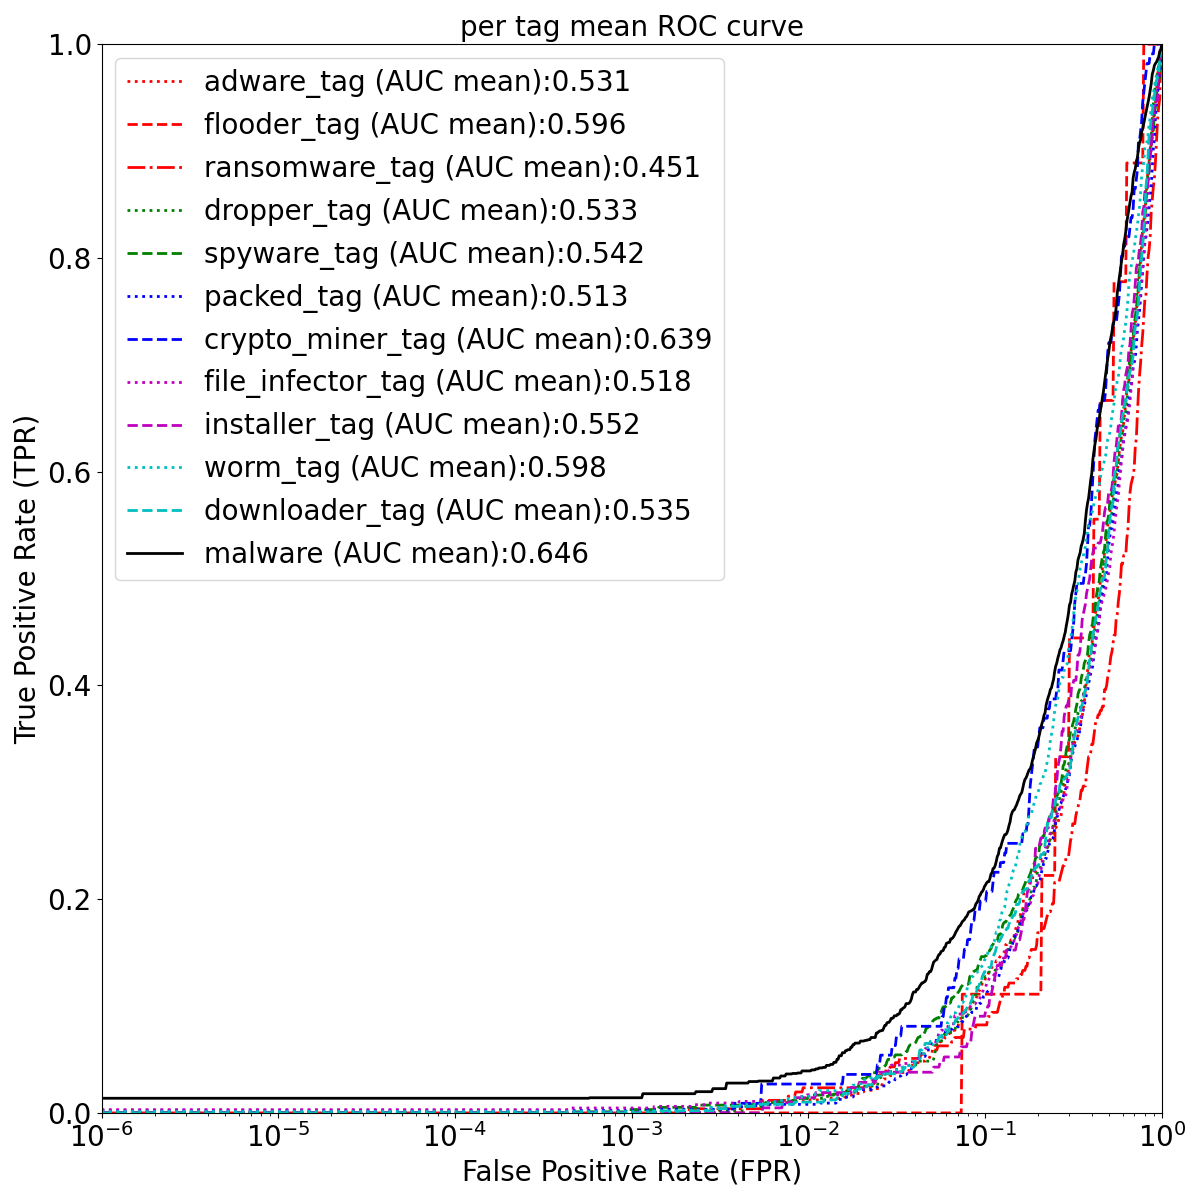
\includegraphics[width=0.6\textwidth]{./results/all_mean_roc_aloha.png}
        \vspace*{-0.2cm}
        \caption[Tags prediction task ALOHA mean ROC curve]{Mean ROC curve and AUC statistics of \textBF{ALOHA} model for the tags/labels. The line represents the \textit{mean} TPR at a given FPR. Statistics were computed over \textBF{2} training runs, each with random parameter initialization.}
        \label{fig:allMeanRocAloha}
    \end{figure}
}

\newcommand{\allMeanRocJointEmbedding}{
    \begin{figure}[H]
        \vspace*{-0.5cm}
        \centering
        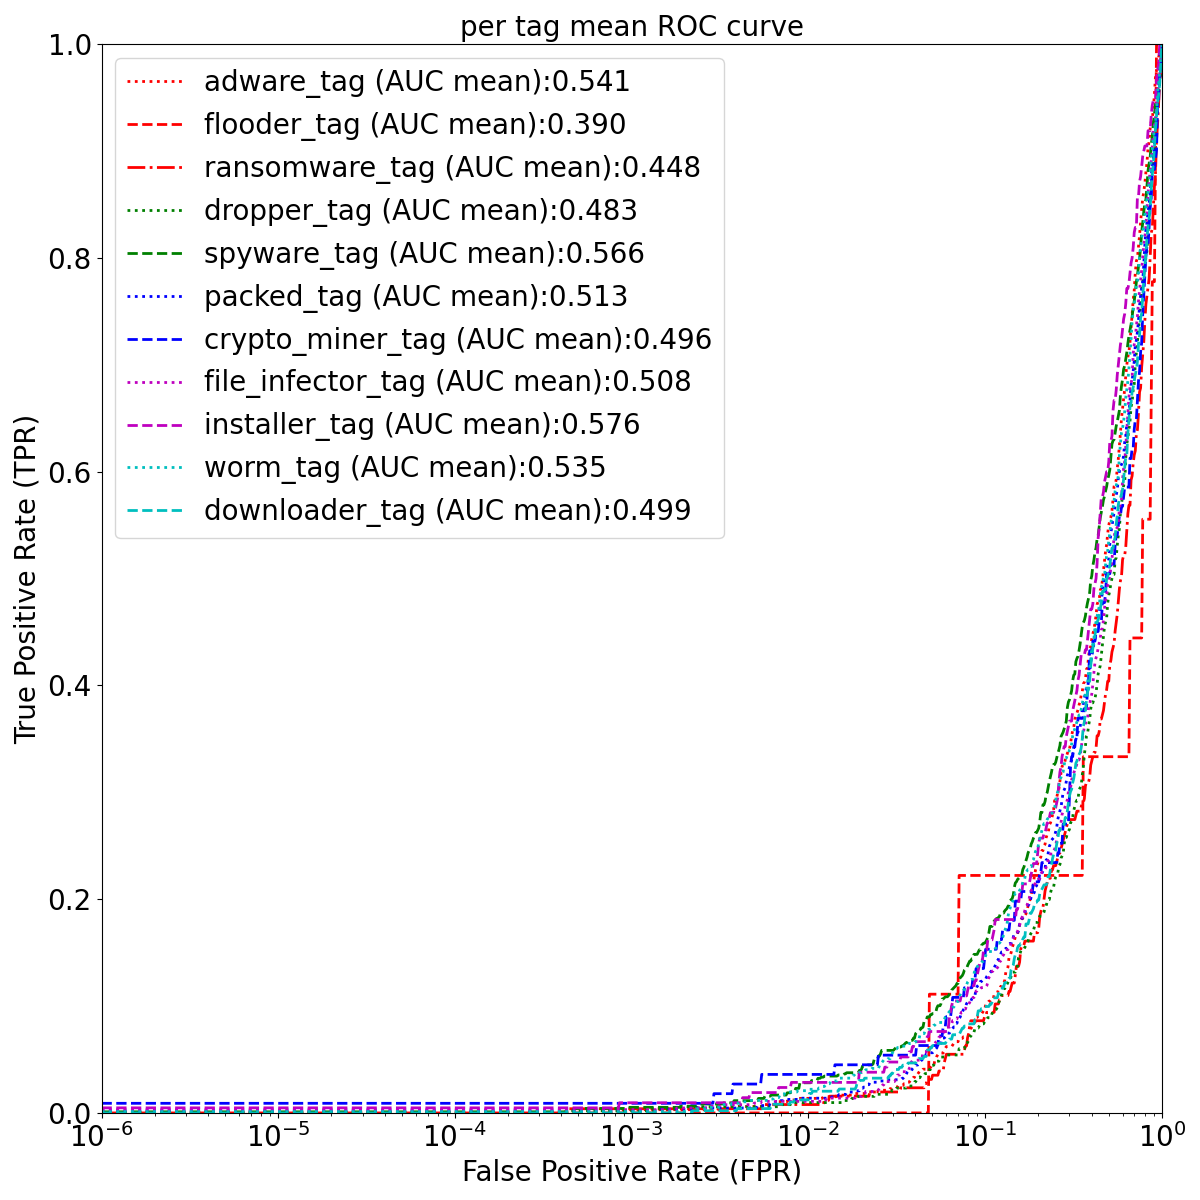
\includegraphics[width=0.6\textwidth]{./results/all_mean_roc_jointEmbedding.png}
        \vspace*{-0.2cm}
        \caption[Tags prediction task Joint Embedding mean ROC curve]{Mean ROC curve and AUC statistics of \textBF{Joint Embedding} model for all tags/labels. The line represents the \textit{mean} TPR at a given FPR. Statistics were computed over \textBF{2} training runs, each with random parameter initialization.}
        \label{fig:allMeanRocJointEmbedding}
    \end{figure}
}

\newcommand{\allMeanRocProposedModel}{
    \begin{figure}[H]
        \vspace*{-0.5cm}
        \centering
        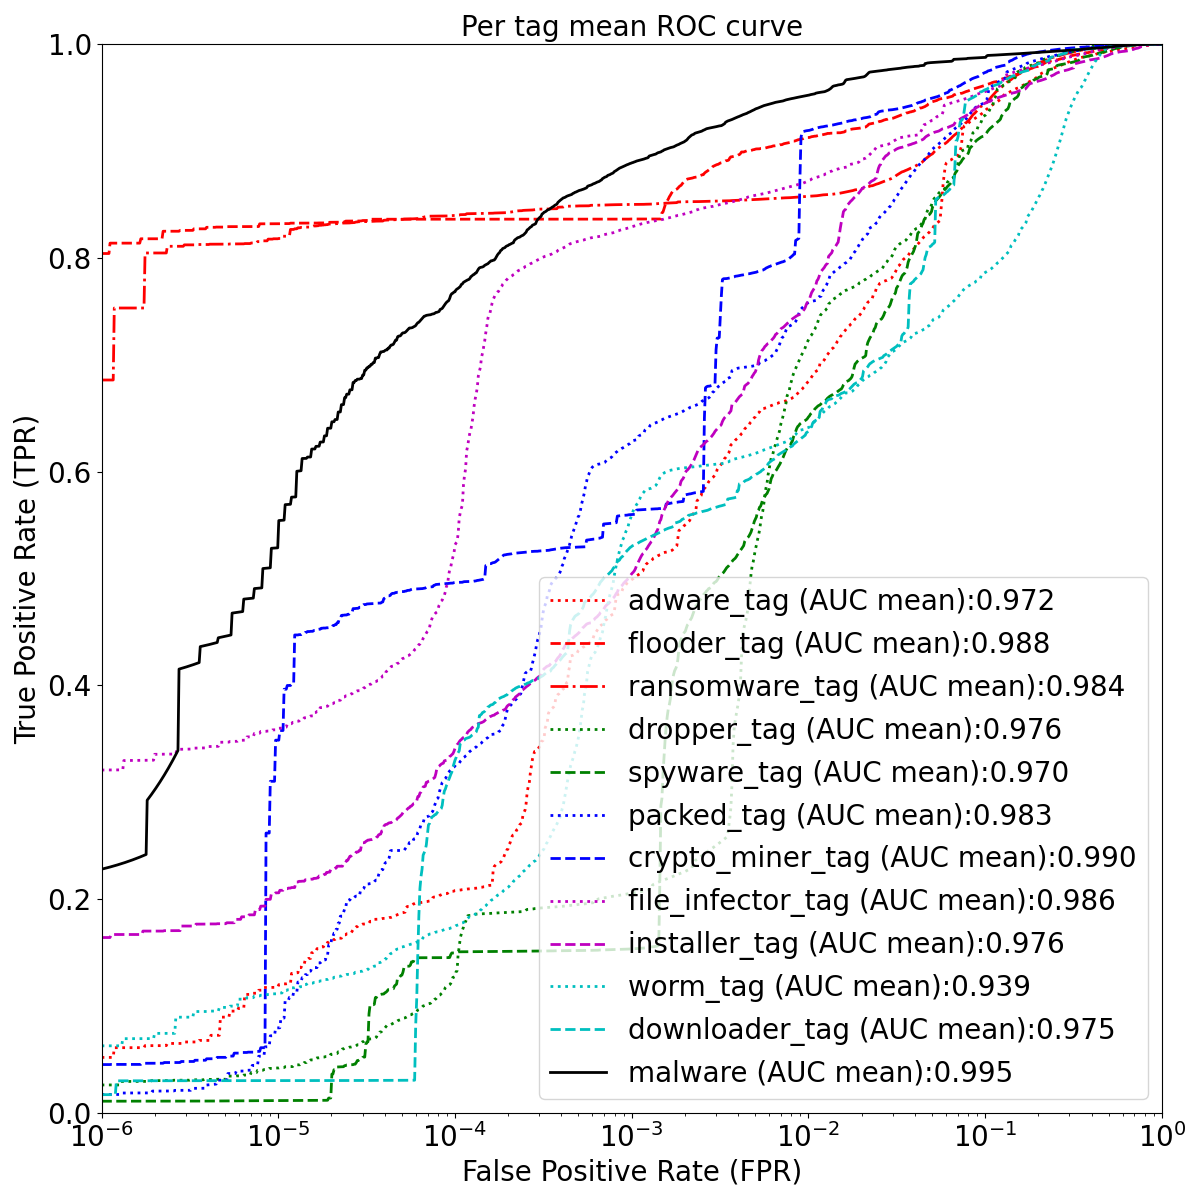
\includegraphics[width=0.6\textwidth]{./results/all_mean_roc_proposedModel.png}
        \vspace*{-0.2cm}
        \caption[Tags prediction task Proposed Model mean ROC curve]{Mean ROC curve and AUC statistics of \textBF{Proposed Model} for the tags/labels. The line represents the \textit{mean} TPR at a given FPR. Statistics were computed over \textBF{2} training runs, each with random parameter initialization.}
        \label{fig:allMeanRocProposedModel}
    \end{figure}
}